%%
%%
%%      SECTION: BEAM PATTERN 
%%

%% [intro]
%%________________________________________________________

The NIKA2 beam pattern mainly depends on the IRAM 30m telescope and NIKA2 internal optical system characteristics, whereas the detectors themselve might have an impact at sub-dominant level (through e.g. time constants or correlated noises). In this section, first we reconstruct the focus surfaces and present the optimal focus, then we characterize both the main beam, which is modeled as an elliptical Gaussian, and the full beam pattern including error beams up to angular scales of 10 arcmin. 

%% [Optimal Focus]
%%________________________________________________________
\subsection{Optimal focus}
\label{sec:focus}

Owing to the NIKA2 $6.5~\rm{arcmin}$ FOV, the focus is expected to
slightly changes across the FOV, defining curved focal surfaces at the
location of the three arrays. Therefore, beam patterns are expected to
show some scatter across the FOV accordingly to the focal
surfaces. Although all the detectors cannot be individually focalised,
an optimal axial focus of the telescope can be found to maximize the
number of detectors at the best focus and hence, maximize the
resolution of the NIKA2 maps. This optimal z-focus setting is obtained
in measuring the focus at the center of the arrays as described
Sect.~\ref{sec:focus-meas} and apply a focus shift, which is primary
predicted using Zemax simulation, and ultimately verified by measuring
the focus surfaces, as decribed in Sect.~\ref{sec:focus-surf}.


\subsubsection{Focus estimation}
\label{sec:focus-meas}

The best axial focus in the central region of the arrays is estimated
using the so-called 'focus$\_$OTF' PAKO script, which realises a
series of five $1' \times 5'$ OTF scans at various values of
the focus in $0.4~\rm{mm}$-steps around an \emph{a priori} value $z_0$,
namely $z \in \{-0.8, -0.4, 0, 0.4, 0.8\} + z_0$. Elliptical Gaussian
fit on the reconstructed maps provide estimates of the flux and FWHM
along minor- and major-axis for each focus. Then, parabolic fits are
used to determine the best focus. We consider three estimates: i)
$\hat z_{\rm{peak}}$ the focus that maximizes the estimated flux,
which is the amplitude of the 2D Gaussian, 
ii) $\hat z_{\rm{fwhm}}$ the focus that
minimizes the geometrical FWHM, defined as the quadratic mean of
$\rm{FWHM}_{\rm{major}}$ and $\rm{FWHM}_{\rm{minor}}$,  and iii)
$\hat z_{\rm{ellipt}}$ the focus that minimizes the beam ellipticity,
defined as $\rm{FWHM}_{\rm{major}}/\rm{FWHM}_{\rm{minor}}$.
Fig.~\ref{fig:focus-example} shows an example of
axial focus measurement using a 'focus$\_$OTF' observation of Neptune
during N2R10.

\begin{figure}
\begin{center}
  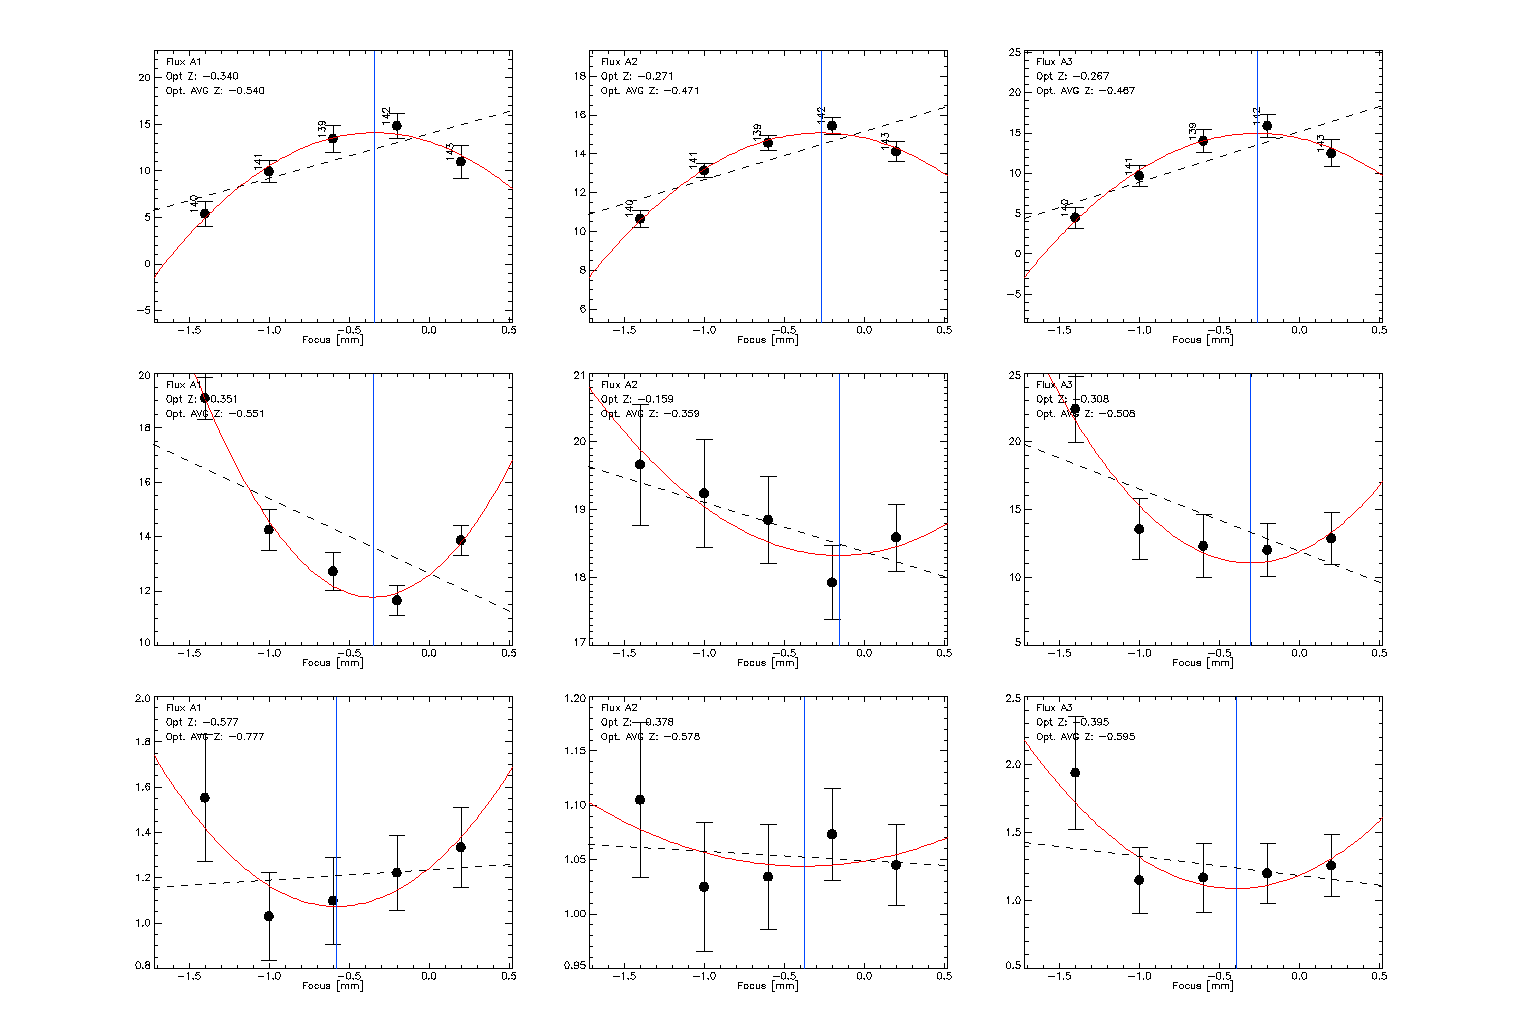
\includegraphics[clip, angle=0, scale=0.25]{Figures/plot_20170419s143.png}
\caption{Example of axial focus measurment using a 'focus$\_$OTF' observation of Neptune
during N2R10 [PLACEHOLDER]}
\label{fig:focus-example}
\end{center}
\end{figure}


\subsubsection{Reconstruction of the focus surfaces}
\label{sec:focus-surf}

\begin{figure}
\begin{center}
  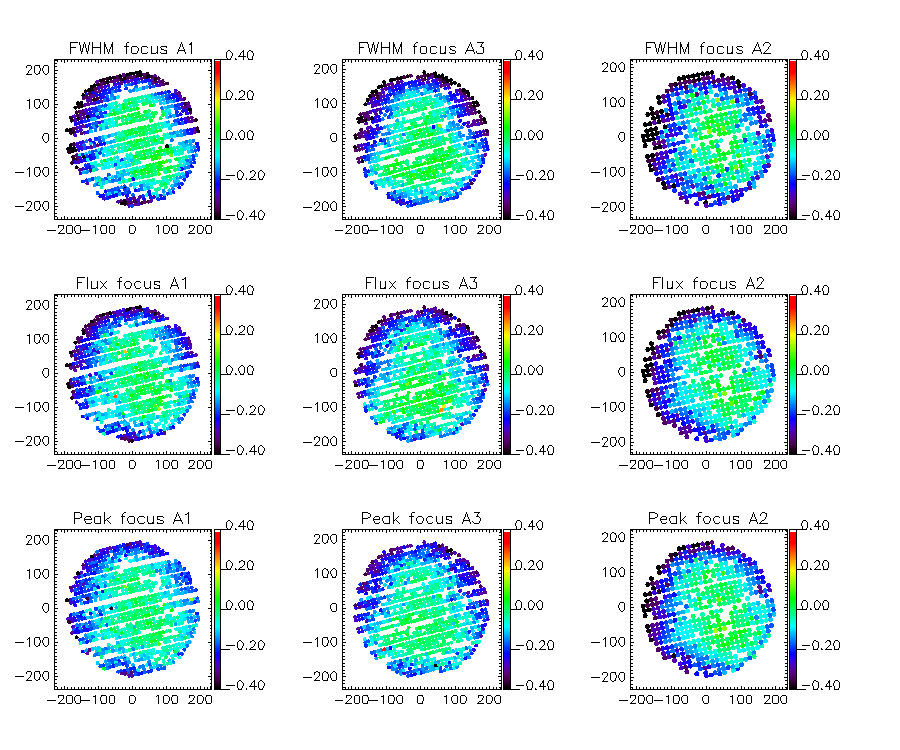
\includegraphics[trim={0, 1cm, 0, 1cm}, clip, angle=0, scale=0.5]{Figures/fov_focus_mv_5.png}
\caption{Focus surface of A1, A3 and A2 arrays from left to
  right. From top to bottom, the focus estimates rely on
  FWHM-minimization, amplitude-maximization of an elliptical
  Gaussian of fixed FWHMs and amplitude-maximization of an elliptical
  Gaussian.}
\label{fig:focus-surfaces}
\end{center}
\end{figure}

\emph{Method. } We measure NIKA2 focal surfaces by means of a sequence of five 'beam-map'
scan observations of bright point-like sources, typically Planets or
bright quasars,
for various settings of the telescope axial focus around the
optimal focus $z_{\rm{opt}}$. A beam-map scan consists of a deep-integrated
$13.5' \times 7.8'$ OTF-scan observation comprizing $99$ sub-scans and
with a scanning speed of $39''/s$ [TBC]. The z-focus is changed in step of
$0.6~\rm{mm}$ to probe a large focus range for measuring even the
extreme variation of the focus surfaces,
namely $z \in \{-1.2, -0.6, 0, 0.6, 1.2 \} + z_{\rm{opt}}$.
Each beam-map scans allow for $4''$-resolution individual maps per kid to
be projected. Before the projection, the correlated noise is mitigated
from each KID timeline in subtrating out a common mode, which is obtained
using, amongst the other detectors, those that correlates the most
with this KID and that are located outside a radius of $90''$
around the source centroid.
Therefore, a series of five cleaned maps at various focus is
available for each detector, from which the best focus is estimated as
described in Sect.~\ref{sec:focus-meas}. The ensemble of the relative
focus estimate per KIDs with respect to the best focus at the center
of the array constitutes the focus surface. An accurate estimate of
the center focus is obtained as the
weighted average focus estimate of the KIDs lying in a $30''$ radius
around the geometrical center of the array. This average does not
induce any sizeable bias thanks to the flatness of the focus surface
in the innermost regions. For robustness test, we consider three focus
estimates: the two first ones are the same as discussed in
Sect.~\ref{sec:focus-meas} -- namely i) $\hat z_{\rm{fwhm}}$ the focus that
minimizes the geometrical FWHM and ii) $\hat z_{\rm{peak}}$ the focus
that maximizes the amplitude of the best-fitting ellitical Gaussian --
whereas the third one is $\hat z_{\rm{flux}}$ the focus that maximizes
the amplitude of the best-fitting elliptical Gaussian of fixed FWHM
(at $12''$ at $260~\rm{GHz}$ and $18''$ at $150~\rm{GHz}$). The 
comparison between the two amplitude-based estimators
($\hat z_{\rm{peak}}$ and $\hat z_{\rm{flux}}$), will test the
stability of the focus results against the exact choice of the beam fitting
function. Since the ellipticity-based estimator $\hat z_{\rm{ellip}}$ is
less sensitive to focus changes and yields larger uncertainties than the
others, we do not use it for the focus surface reconstruction.     


\emph{Data selection. }
During the three commissioning campaigns that occured after the change of A1
lens (hence in the final NIKA2 optic configuration), nine out-of-focus
beam-map scan sequences have been acquired, including incomplete
sequences and sequences hindered by poor atmospheric conditions. We
select sequences that i) comprises at least four scans, ii) have been
observed at zenith opacity at $225~\rm{GHz}$ (as indicated by
the IRAM taumeter) below 0.5 and iii) have a maximal central focus
drift between the starting time and the end of the sequence of
$0.5~\rm{mm}$. These criteria preserve five sequences from which focus
surfaces can be reconstructed. Namely, we consider the sequences
$20170226s415\mbox{--}419$, $20170419s133\mbox{--}137$, $20170420s113\mbox{--}117$,
$20170421s160\mbox{--}164$ and $20170424s123\mbox{--}127$, which consist of observations
of the bright quasar '3C84' and Neptune.

\emph{Results. }
For each detector $k$ and each beam-map sequence $s$, we obtain for
the array $a$, a focus measurement $z_k^{a, s} \pm \sigma_k^{a, s}$,
where $\sigma_k^{a, s}$ is the $1\mbox{--}\sigma$ error of the least-square
polynomial fit. The focus surface measurements per arrays obtained from the five
beam-map sequences are combined using an inverse-variance weighting
scheme to obtain the focus surface estimates 
\begin{equation}
\label{eq:mv_focus_surf}
z_k^{(a)} = \left( \sigma_k^{(a)} \right)^2 \,  \sum_s \frac{z_k^{a,s}}{\left(\sigma_k^{a,s}\right)^2}\, \,  ,
\end{equation}
with uncertainties 
\begin{equation}
\label{eq:error_mv_focus_surf}
\sigma_k^{(a)} = \left[ \sum_s \frac{1}{\left(\sigma_k^{a,s}\right)^2}\right]^{-1/2}\, .
\end{equation}


We present NIKA2 focus surfaces per arrays obtained as in
Eq.~\ref{eq:mv_focus_surf} 
%from the inverse-variance weighted combination of the five
%reconstructed focus surfaces per arrays
in Fig.~\ref{fig:focus-surfaces}.
The three flavours of focus-estimators provide us with focus surfaces
per arrays that are in good agreement with each others and that have a
non-axisymetrical flatten bowl shape consistent with expectations from
simulation [TBA, as discussed further below].
The median defocus (that is the relative focus w.r.t. the center)
across the detectors is of about
$-0.1~\rm{mm}$ for the three arrays. Maximal defocus values of about
$-0.6~\rm{mm}$ are found for detectors located in the outer top and
left regions of the FOV. Finally, a fraction comprised between $20$
and $30\%$ of the KIDs has a relative $z\le -0.2~\rm{mm}$.  

We primarily estimate the uncertainty of the focus
surface measurements using the standard deviation between the three
estimators $z_k^{(a)}|_{\rm{fwhm}}$, $z_k^{(a)}|_{\rm{peak}}$ and
$z_k^{(a)}|_{\rm{flux}}$. We found approximatively homogeneous
standard deviation surfaces per arrays, which have median values across
the FOV of about $0.03~\rm{mm}$.
However, we cross-check this error estimate by forming the quadratic mean of
the three inverse-variance error surfaces per arrays, which are defined in
Eq.~\ref{eq:error_mv_focus_surf} and quoted
$\sigma_k^{(a)}|_{\rm{fwhm}}$, $\sigma_k^{(a)}|_{\rm{peak}}$ and
$\sigma_k^{(a)}|_{\rm{flux}}$. This provides us with more optimistic
error surfaces per array, which do not show any clear pattern across
the FOV and which have a median value across the detectors of about
$0.015~\rm{mm}$.  


[EXPAND THE DISCUSSION ON COMPARISON WITH SIMULATION]

\emph{Stability across sequences. }
By comparing the focus surface obtained from the five individual focus
sequences, we test the stability of the NIKA2 focus surfaces across
the time and the atmospheric conditions. In
Figs.~\ref{fig:focus-stability-H}-\ref{fig:focus-stability-V}, we compare
the defocus along two perpendicular diameters across the
FOV. Although any direction would have been equivalent for this test, we choose to
position the diameters along-with and perpendicular-to the KID geometrical
grid to avoid the scatter due to KID non-alignement in any other
direction. The scatter is further mitigated by considering
four-detector-wide diameters as shown in upper the left corner of
Figs.~\ref{fig:focus-stability-H}-\ref{fig:focus-stability-V}.

[DEVELOP A LITTLE THE DISCUSSION HERE]

\begin{figure}
  %\begin{center}
  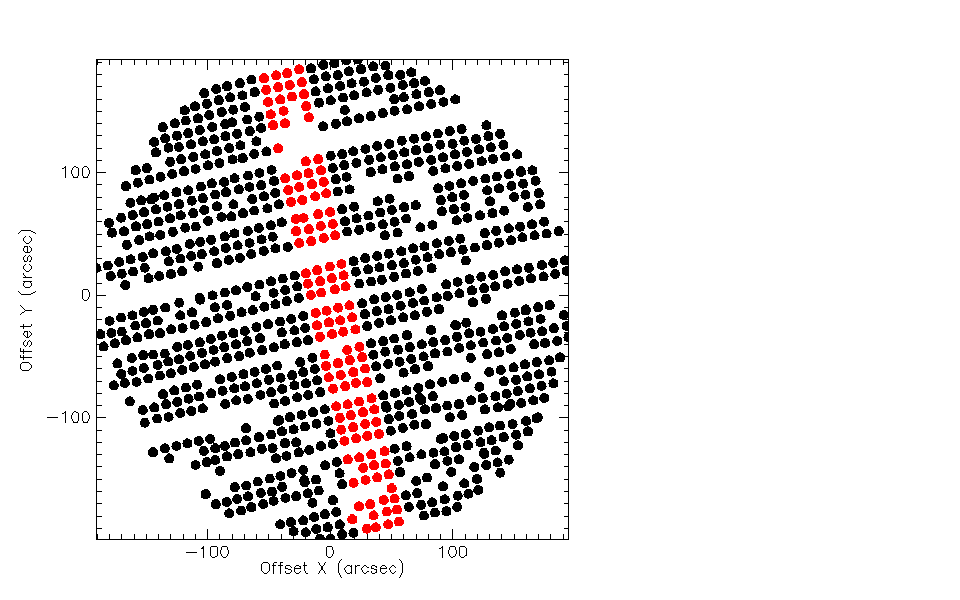
\includegraphics[trim={-2cm, 2cm, 0, 2cm}, clip, angle=0, scale=0.1]{Figures/fov_focus_stability_check_D1.png}
  \begin{center}
  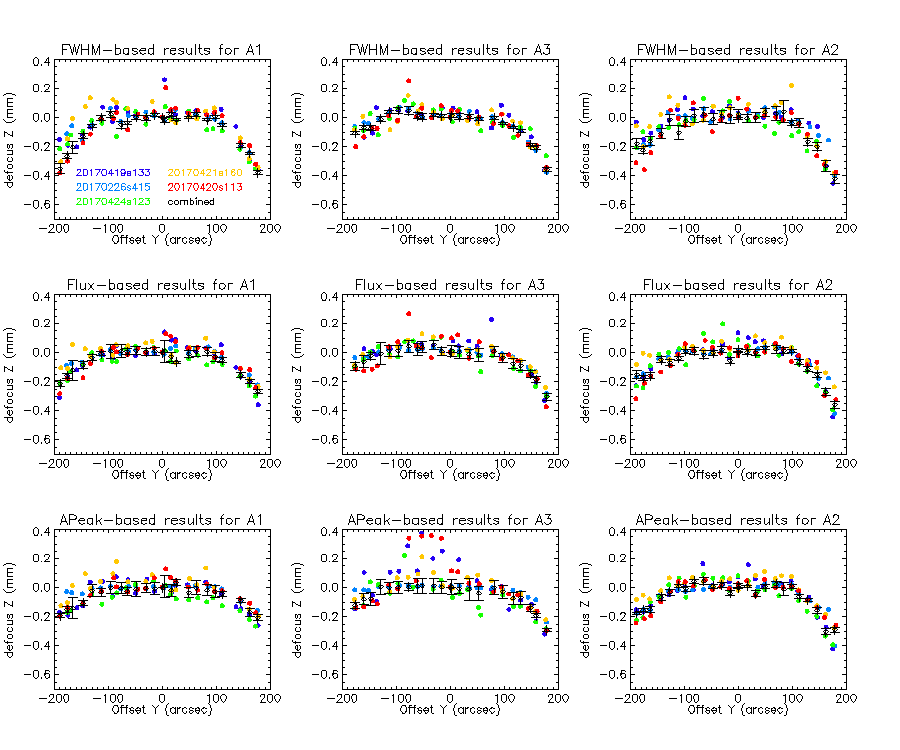
\includegraphics[trim={0, 2cm, 0, 2cm}, clip, angle=0, scale=0.45]{Figures/fov_focus_1D_Vband_5.png}
  \end{center}
  \caption{Stability of the focus surface across the sequences. This
    series of plot show the relative focus with respect to the center
    (defocus) along the 'vertical diameter', that is a band of
    four-detector width across the FOV, which is vertical with respect to
    the detector geometrical grid, as illustrated by the plot in the
    upper left corner. The datapoints show the defocus along the
    'vertical diameter' estimated from the five focus sequences,
    namely $20170226s415\mbox{--}419$ (sky blue),
    $20170419s133\mbox{--}137$ (dark blue), $20170420s113\mbox{--}117$ (red),
    $20170421s160\mbox{--}164$ (yellow) and $20170424s123\mbox{--}127$
    (green), using the $z^{(a)}|_{\rm{fwhm}}$, $z^{(a)}|_{\rm{flux}}$ and
    $z^{(a)}|_{\rm{peak}}$ estimators from top to bottom, and for A1, A3 and
    A2 arrays from left to right. The black datapoints are the five-sequence combined defocus, as
    presented in Fig.~\ref{fig:focus-surfaces}, taken along the
    'vertical diameter', and the errorbars, the
    five-sequence combined defocus errors along the 'vertical
    diameter'.}
\label{fig:focus-stability-H}
\end{figure}


\begin{figure}  
  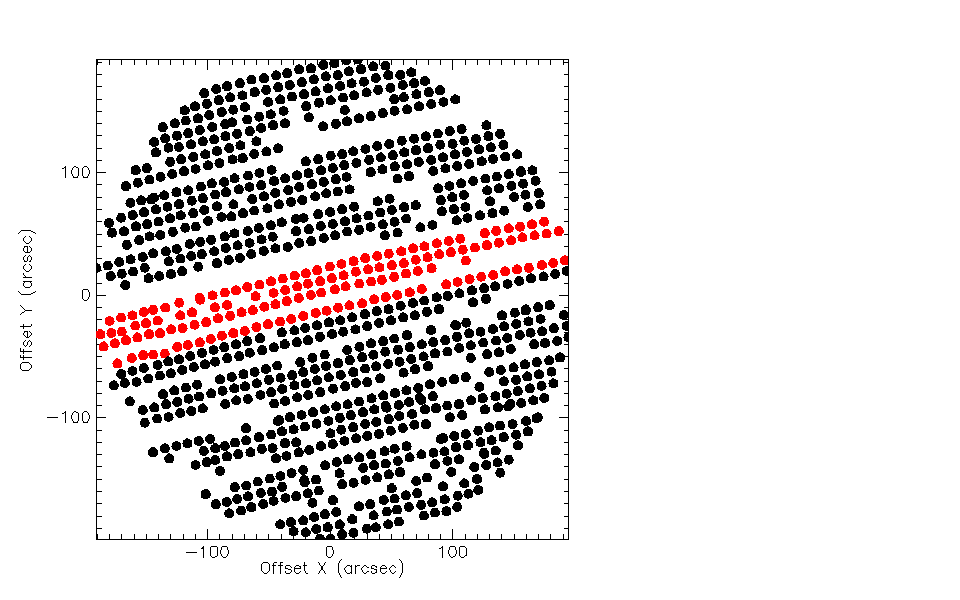
\includegraphics[trim={-2cm, 2cm, 0, 2cm}, clip, angle=0, scale=0.1]{Figures/fov_focus_stability_check_D2.png}
  \begin{center}
  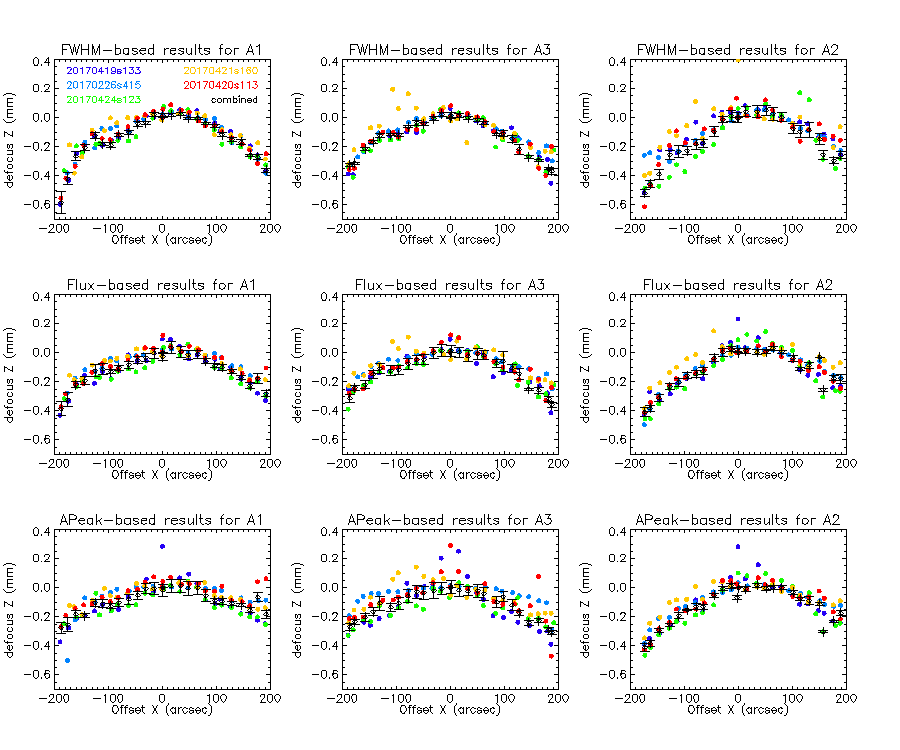
\includegraphics[trim={0, 2cm, 0, 2cm},clip, angle=0, scale=0.45]{Figures/fov_focus_1D_Hband_5.png}
  \caption{Stability of the focus surface across the sequences. Same
    legend as in Fig.~\ref{fig:focus-stability-H}, but for the
    detectors located in an 'horizontal diameter', i.e. a band of
    four-detector width across the FOV, which is horizontal with respect to
    the detector geometrical grid, as illustrated by the plot in the
    upper left corner. }
\label{fig:focus-stability-V}
\end{center}
\end{figure}



%% [Main beam]
%%________________________________________________________
\subsection{Main beam}

For NIKA2 main beam characterization, we use \emph{Run9} OTF scans of bright point sources, including primary and secondary calibrators. Namely, we consider scans of Uranus, Neptune, 3C273, 3C84, 0316+413, Vesta and MWC349, whereas we avoid CRL2688 and NGC7027, which are slighltly extended. We perform a conservative data selection from the observing conditions by demanding average elevations $\rm{el} \ge 20°$, zenith opacities as estimated by NIKA2 in the 1mm band $\tau_{1\rm{mm}} \le 0.4$, reasonable lateral focus settings $x, y \le 0.5$mm. After selection cuts, our data set includes 130 OTF scans, which consists of a representative sub-sample of a typical NIKA2 observation campaign.    

  
We consider different methods for the main beam characterization: i) Gaussian fits of the beam profile to benefit from the signal-over-noise increase after azimuthally averaging the signal, ii) Elliptical Gaussian fits of the beam map for a better 2D modeling. Cross-checking the outputs from these complementary methods is an important robustess test of our results.   


\subsubsection{profile-based analysis}

[JEAN-FRANCOIS]

\subsubsection{map-based analysis}

NIKA2 main beam two-dimensionnal distribution is modeled using an elliptical Gaussian. We characterize NIKA2 resolution by giving the \emph{FWHM}, defined as
\begin{equation}
  FWHM = 2 \sqrt{2\ln {2}} \sqrt{\sigma_x\sigma_y},
\end{equation}
where $\sigma_x$ and $\sigma_y$ are the Gaussian standard deviation along minor- and major-axis. To avoid the side lobes contamination, we use masked versions of the beam map, in which an annulus of inner radius $r_{\rm{in}}$ and outter radius $r_{\rm{out}}$ is cut out. Whereas $r_{\rm{out}}$ is conservately set to be $100 arcsec$, $r_{\rm{in}}$ can vary to provide the best 2D Gaussian fit. We checked a posteriori that $r_{\rm{in}}$ distributes as $7 \pm 1.5$ arcsec at 1mm and $13 \pm 4$ arcsec at 2mm, in agreement with settings defined in the profile-based analysis.   

Figure~\ref{fig:fwhm_map} shows FWHM distributions obtained from the elliptical Gaussian fit method.


\begin{figure}
\begin{center}
  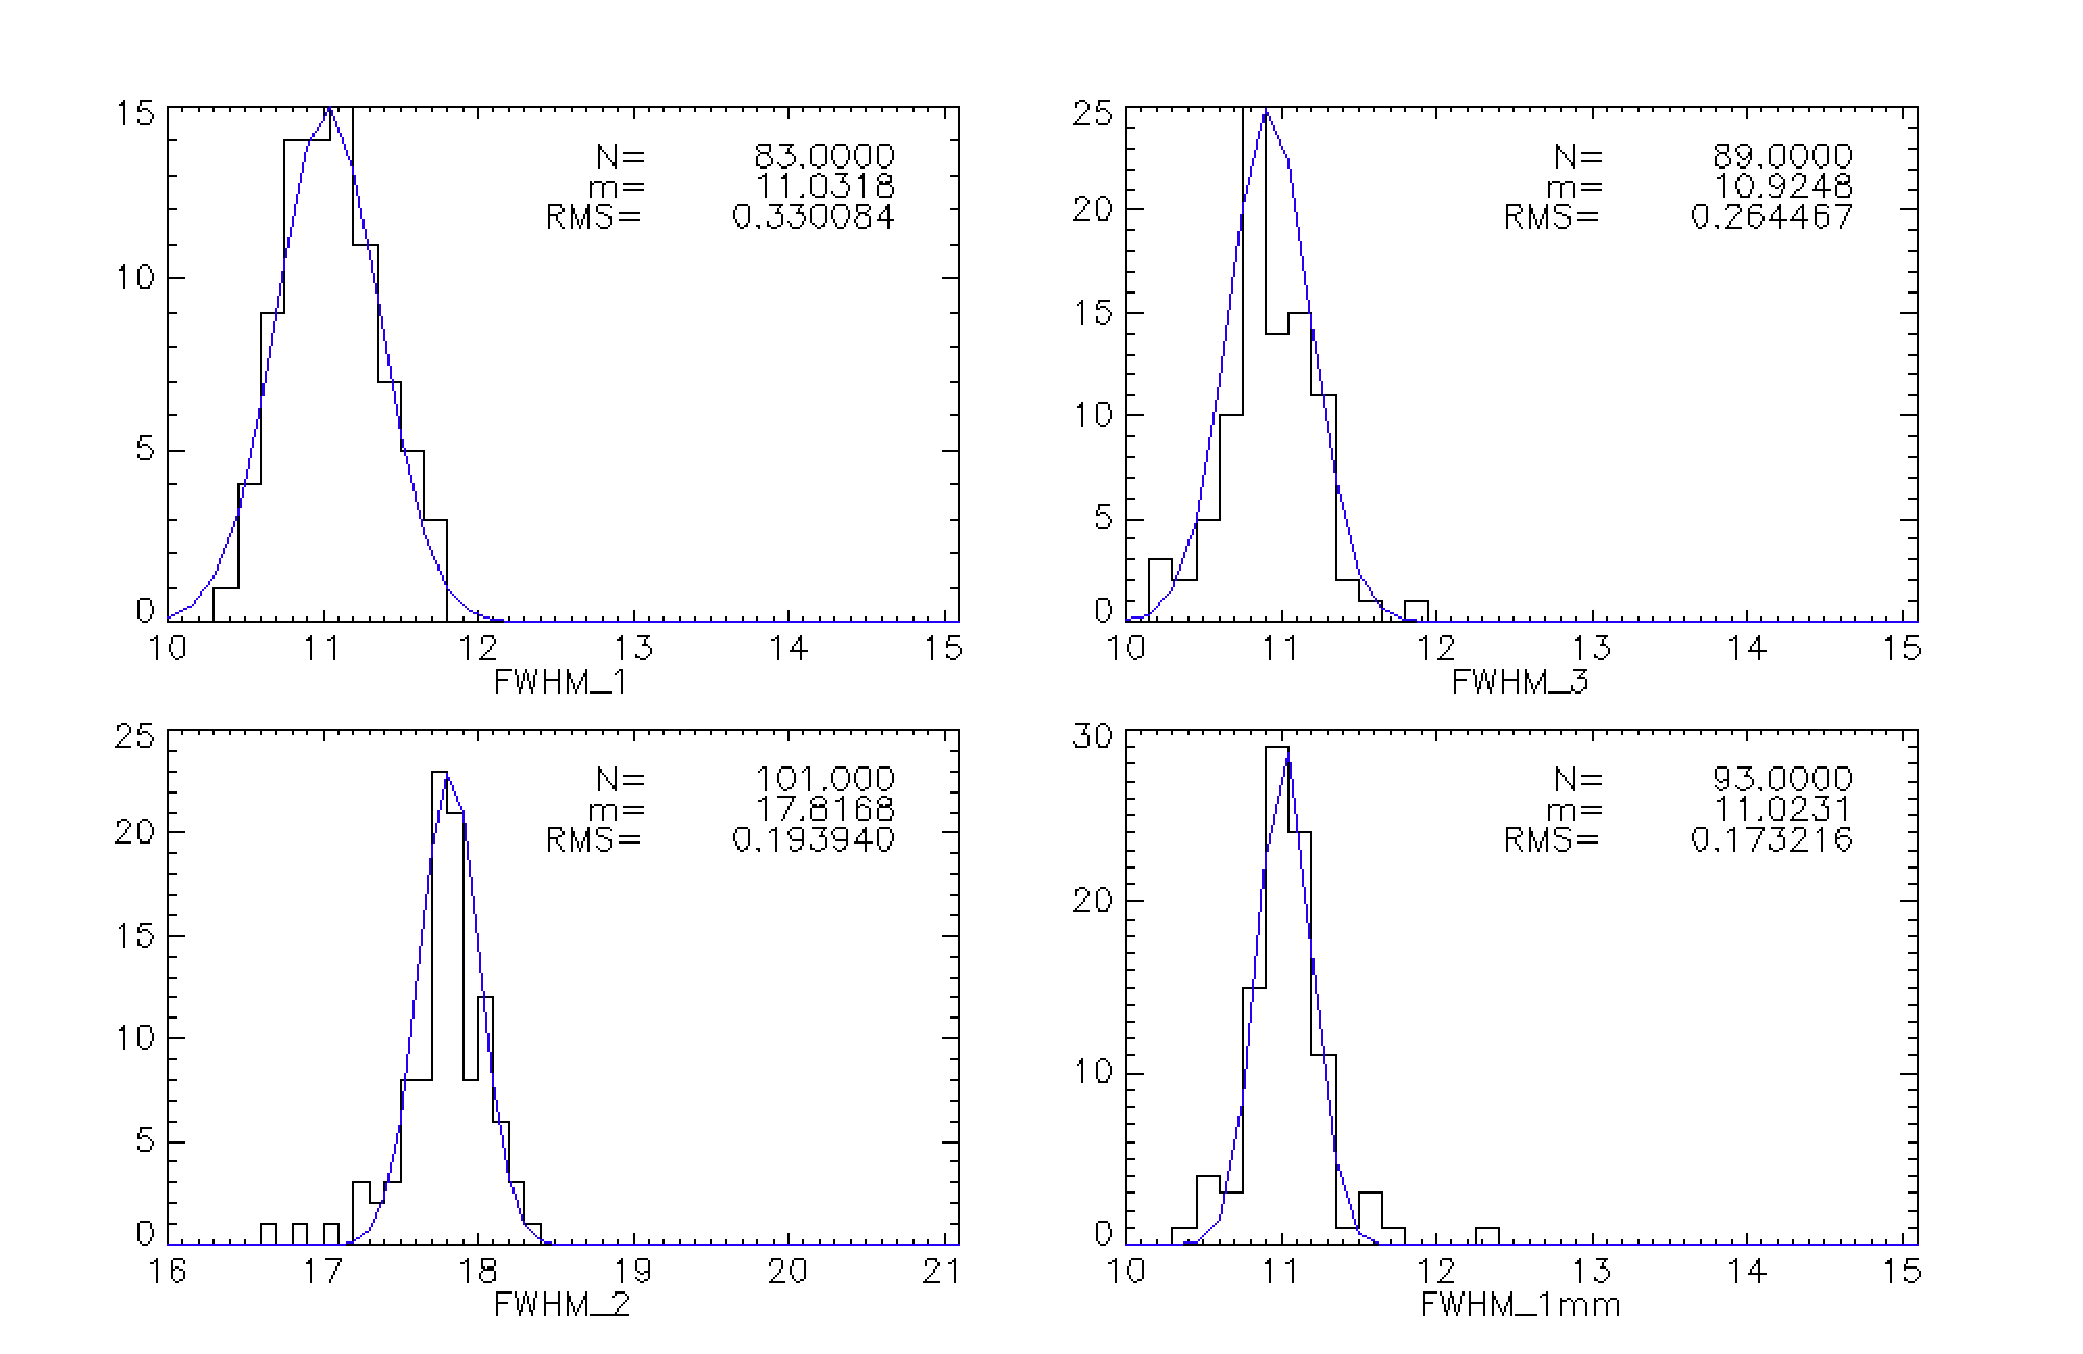
\includegraphics[clip, angle=0, scale=0.4]{Figures/plot_histo_fwhm_run9_calibII_all_nocut.pdf}
\caption{Distribution of the FWHM estimates using 2D Gaussian fits on \emph{N2R9} OTF scans of brigth point sources}
\label{fig:fwhm_map}
\end{center}
\end{figure}


The FWHM estimates using the profile-based and map-based methods are gathered in Tab.~\ref{tab:fwhm}. 
\begin{table}
  \caption[]{FWHM of the NIKA2 main beam in arcsec.}
  \centering
  \begin{tabular}{|l|l|l|l|l|}
    \hline
    Array & profile-based method & map-based method \\
    \hline
    A1       & [TBC] & $11.0 \pm 0.3$ \\
    A3       & [TBC] & $10.9 \pm 0.3$ \\
    A1 \& A3 & [TBC] & $11.0 \pm 0.2$ \\
    A2       & [TBC] & $17.8 \pm 0.2$ \\
    \hline
  \end{tabular}
  \label{tab:fwhm}
\end{table}



%% [Full beam pattern]
%%________________________________________________________
\subsection{Full beam pattern}

\subsubsection{Deep beam maps}
We present the two-dimensional distribution of the beam in Fig.~\ref{fig:beam}. We primary use a map obtained from a combination of deep observations of strong point sources collected during \emph{NIKA2-run8} and \emph{run9}. Namely, we use 'beammap' OTF scans of Uranus (scan id '20170125s223' and '20170125s243'),  Neptune ('20170224s177') and the bright quasar 3C84 ('20170226s415'). However, we checked the stability of our results on single scan maps, combinations of scans for a single source, and combinations of shallower scans but spanning a large range of scanning direction. The data processing includes a mitigation of the correlated noise, which mainly originates from the atmosphere.  We primarly use a subtraction of a common mode estimated from the most correlated detectors (the so-called 'cm one block' method). However, other methods are tested for assessing the immunity of our results to noise residuals.

\begin{figure}
\begin{center}
  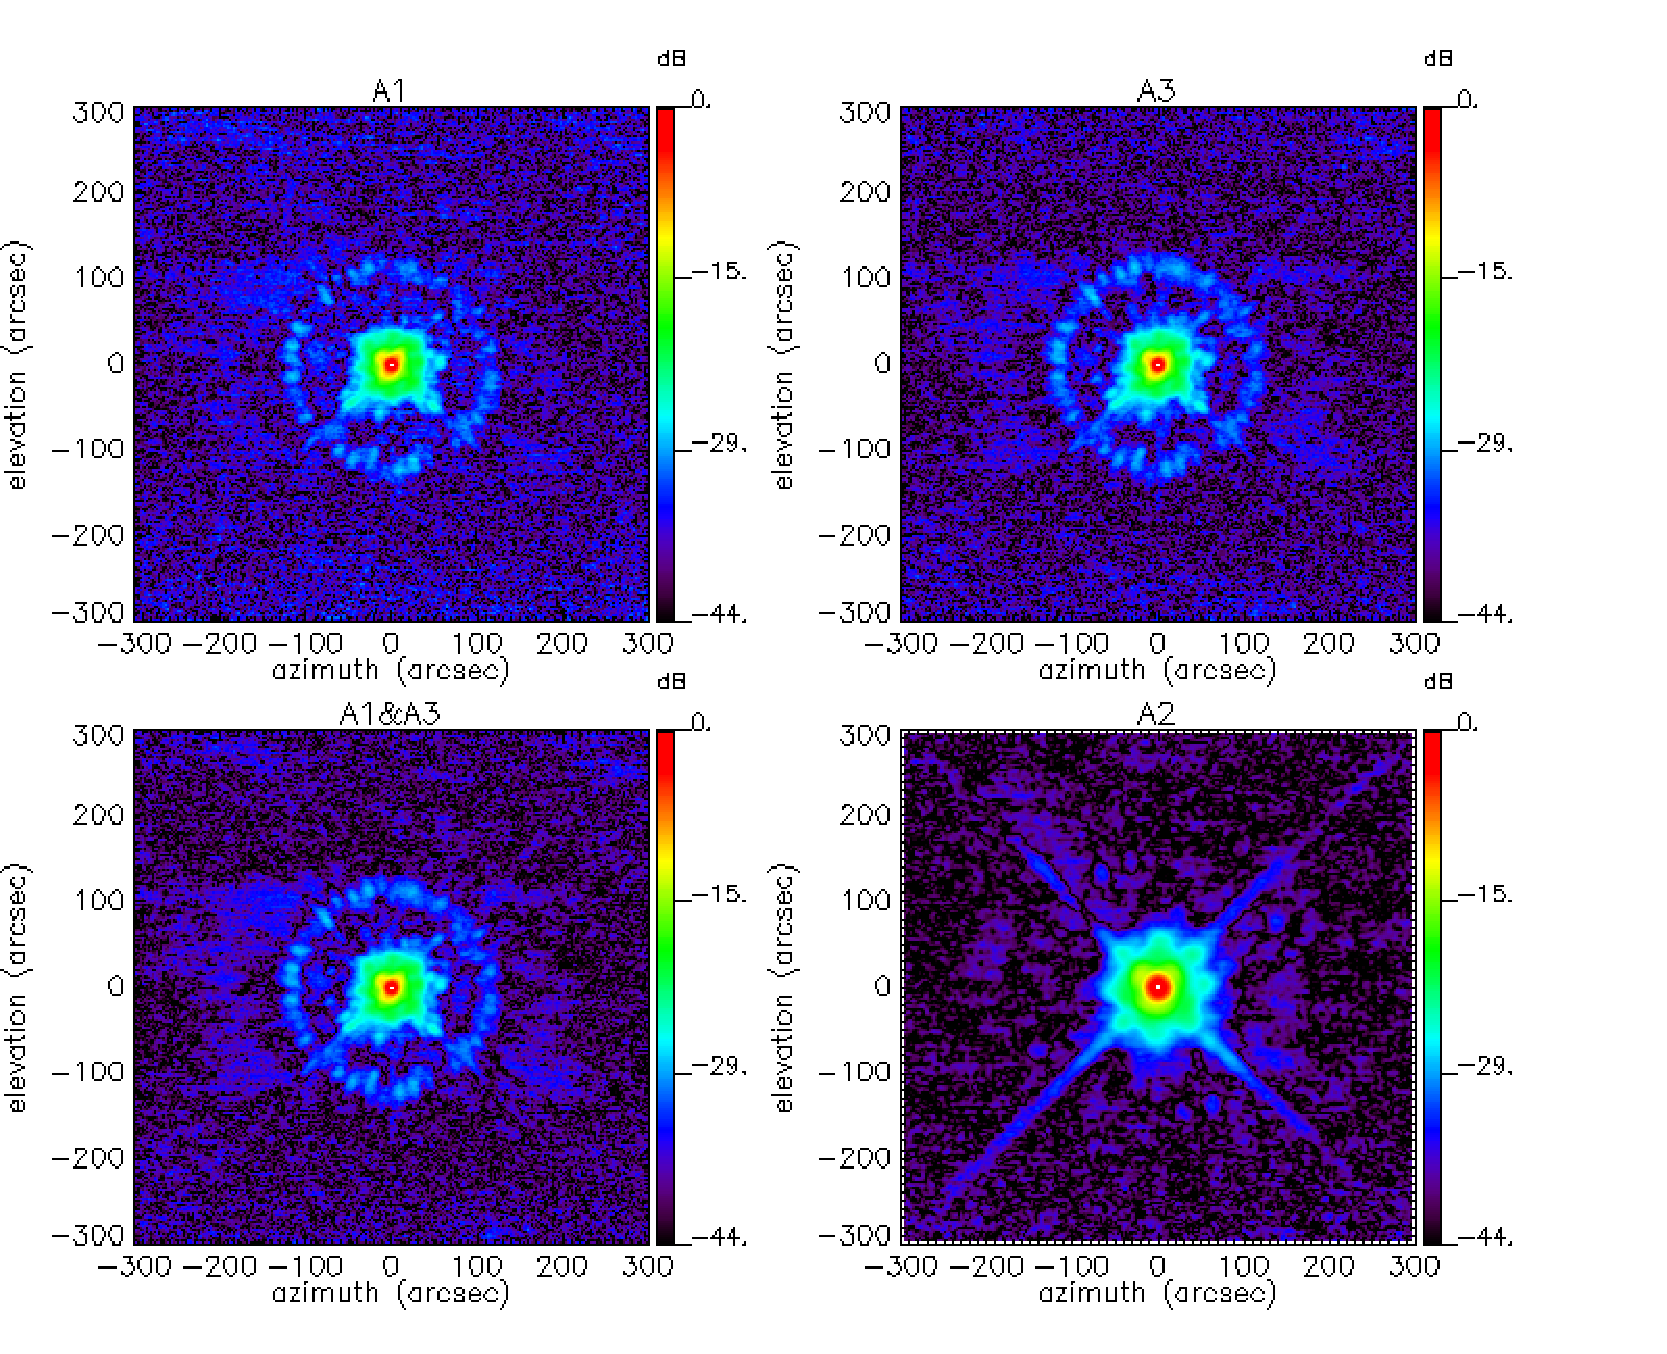
\includegraphics[clip, angle=0, scale=0.4]{Figures/Lobe_map_Combo_v2_dB.pdf}
 \caption{Beam pattern. From upper left to lower right, beam maps of array 1 (labeled 'A1'), array 3 ('A3'), the combination of the 1.15mm arrays ('A1$\&$3') and the 2mm array ('A2') are shown in decibel. These maps, which consist of normalized combination of four long OTF scans of bright point sources, are in celestial coordinates and cover a sky area which extend over 10 arcmin.}
\label{fig:beam}
\end{center}
\end{figure}


The deep NIKA2 beam maps reveal some noticeable features, which are shown in Fig.~\ref{fig:features}. 

\begin{figure}
\begin{center}
  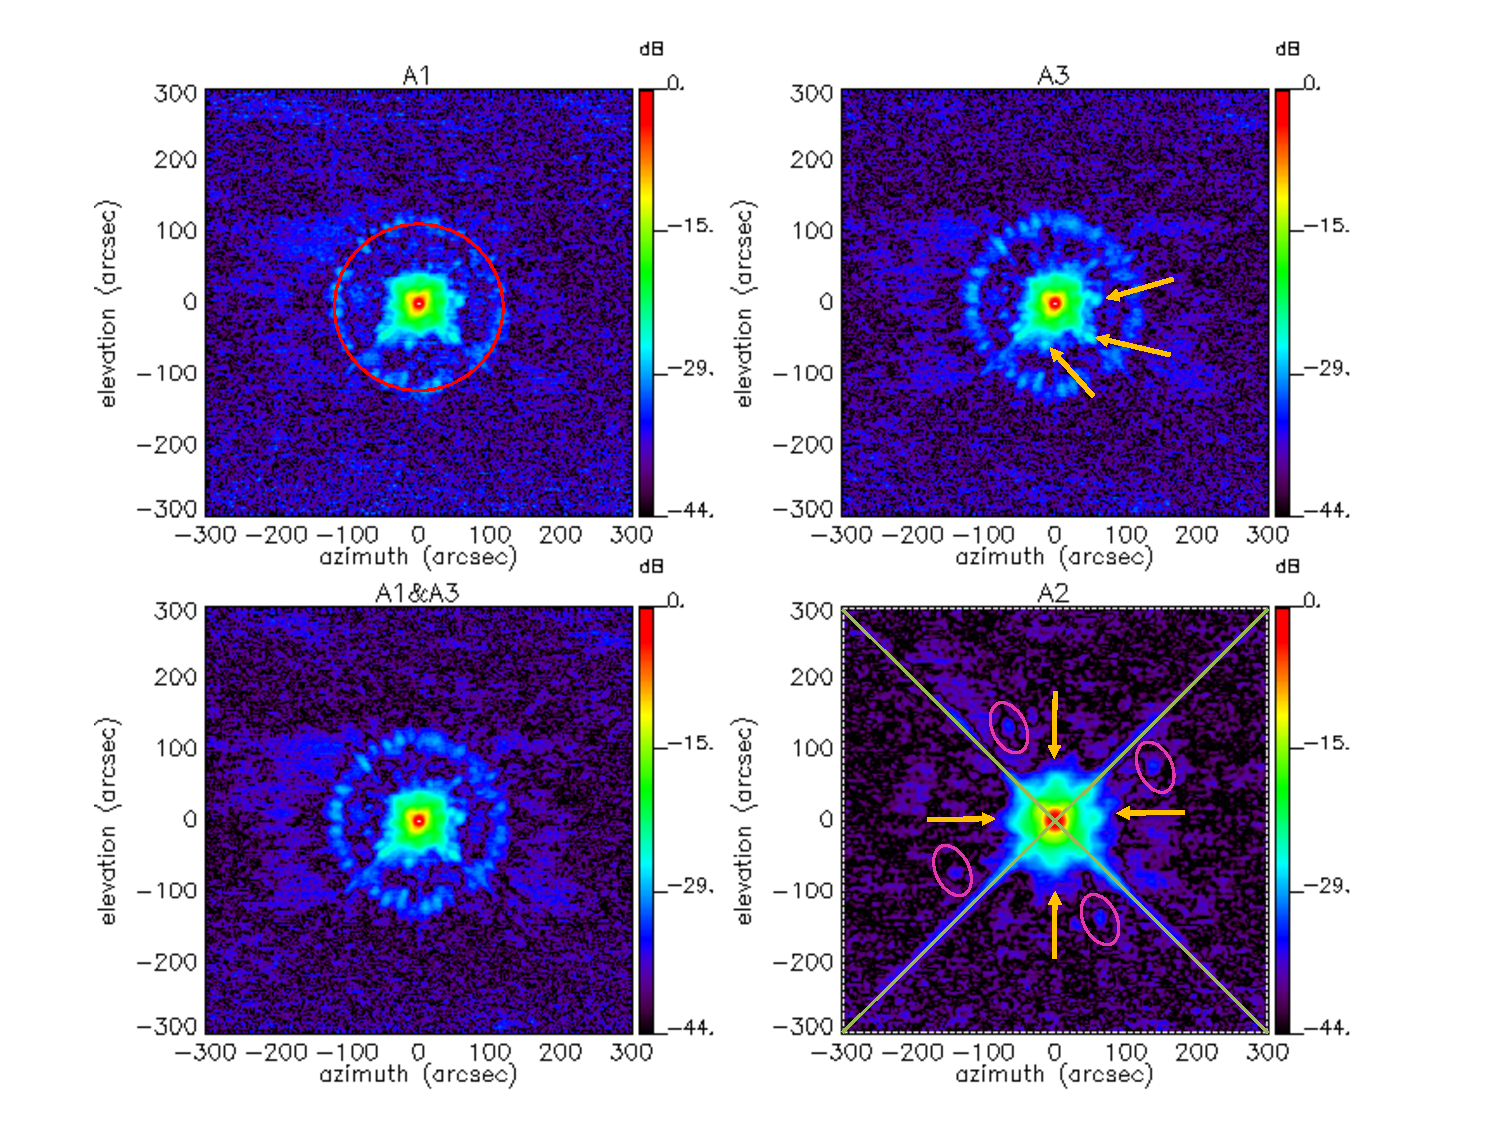
\includegraphics[clip, angle=0, scale=0.4]{Figures/Beams_features.pdf}
\caption{Noticeable features of NIKA2 beam pattern. Red circle: diffraction ring seen in 1-mm maps (the spokes are presumably caused by radial and azimuthal panel buckling (cf. Fig.4 in Greve et al. 2010)); Perpendicular green lines: diffraction pattern caused by quadrupod secondary support structure (prominently seen in 2mm maps); Yellow arrows in the upper right pannel: pattern of 3 spikes seen in 1mm maps of unknown origin; Yellow arrows in the lower right pannel: four symmetrical spokes of the first errorbeam; Pink ellipses: 4 spikes seen in 2mm maps.}
\label{fig:features}
\end{center}
\end{figure}

We further quantify the relative level of the main beam, the first error beam and other features seen in the 2D beam pattern using radial cuts.

[FIGURE JEAN-FRANCOIS]

\begin{figure}
\begin{center}
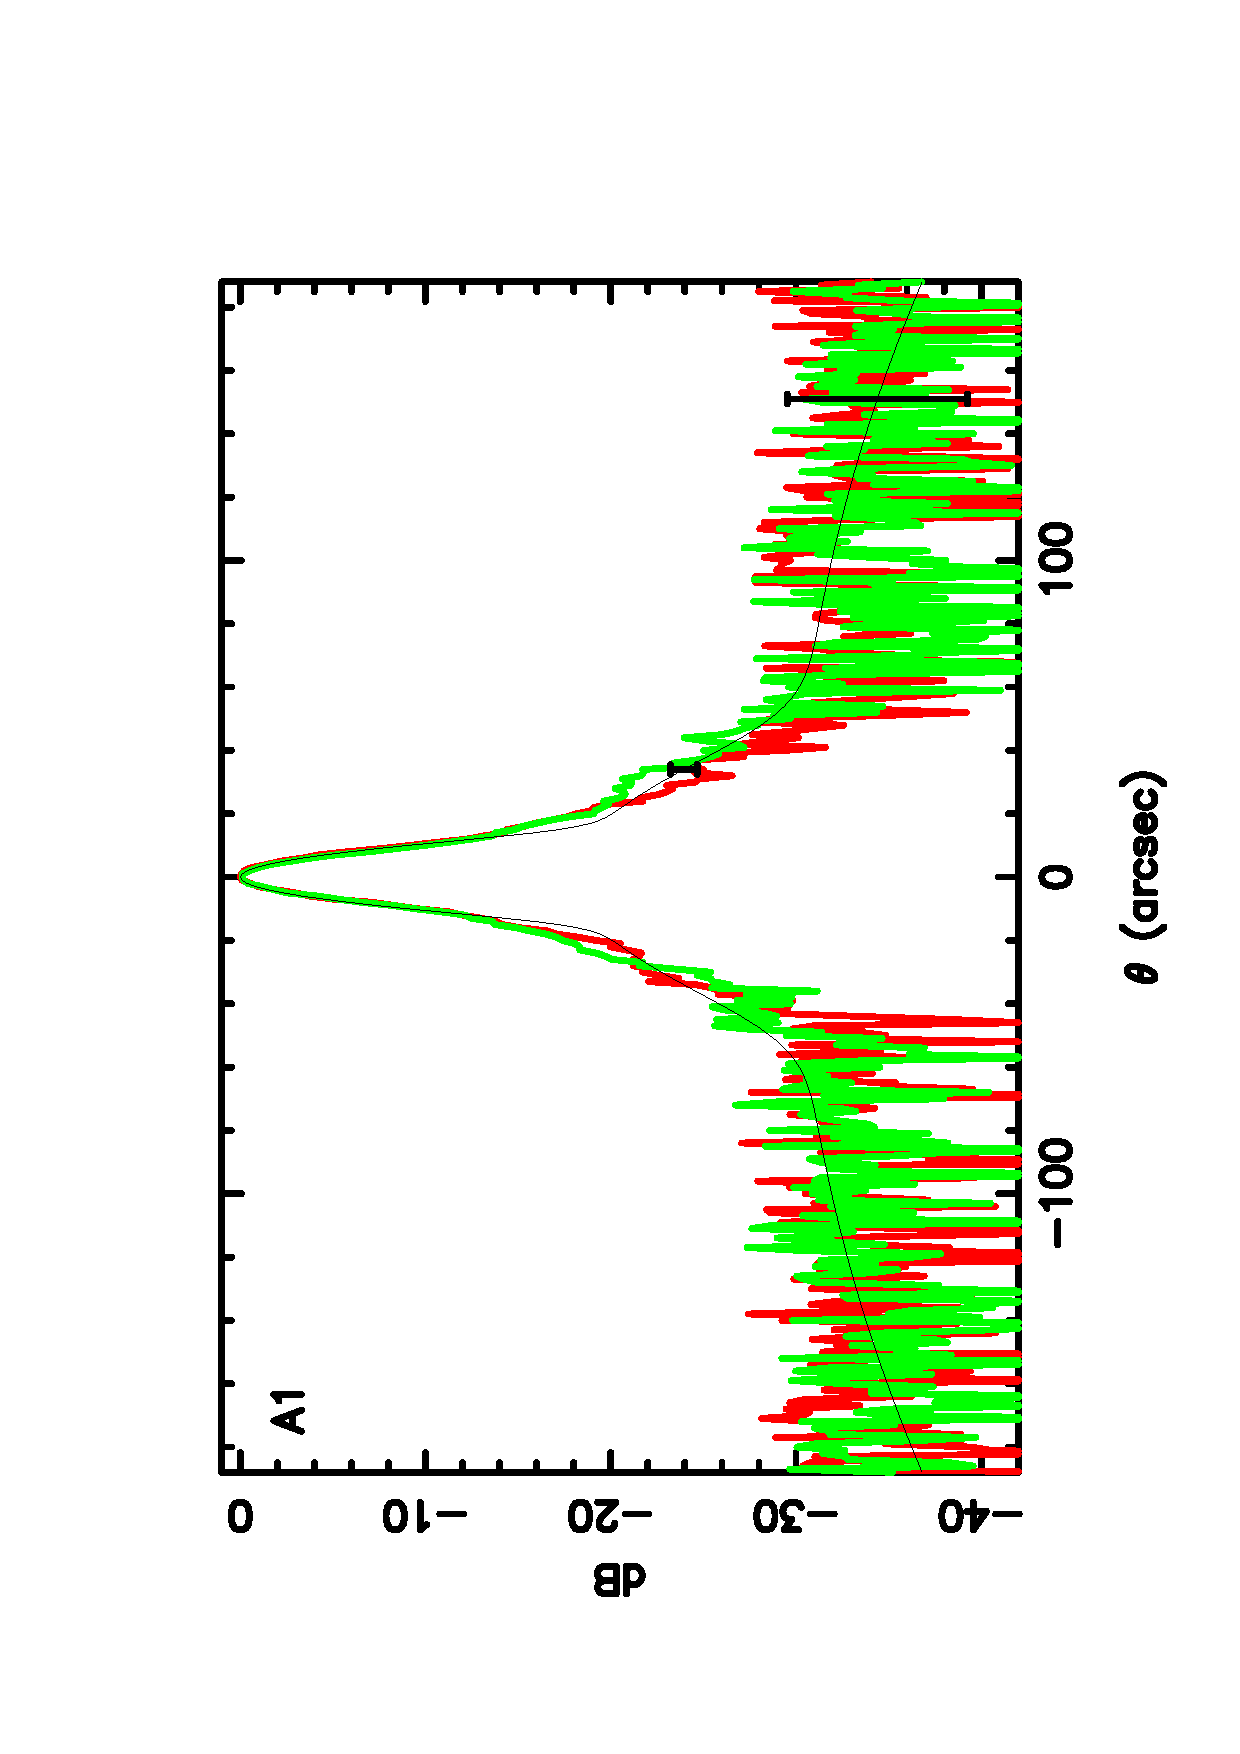
\includegraphics[clip, angle=-90, scale =0.3]{Figures/Array_A1_dB.pdf}
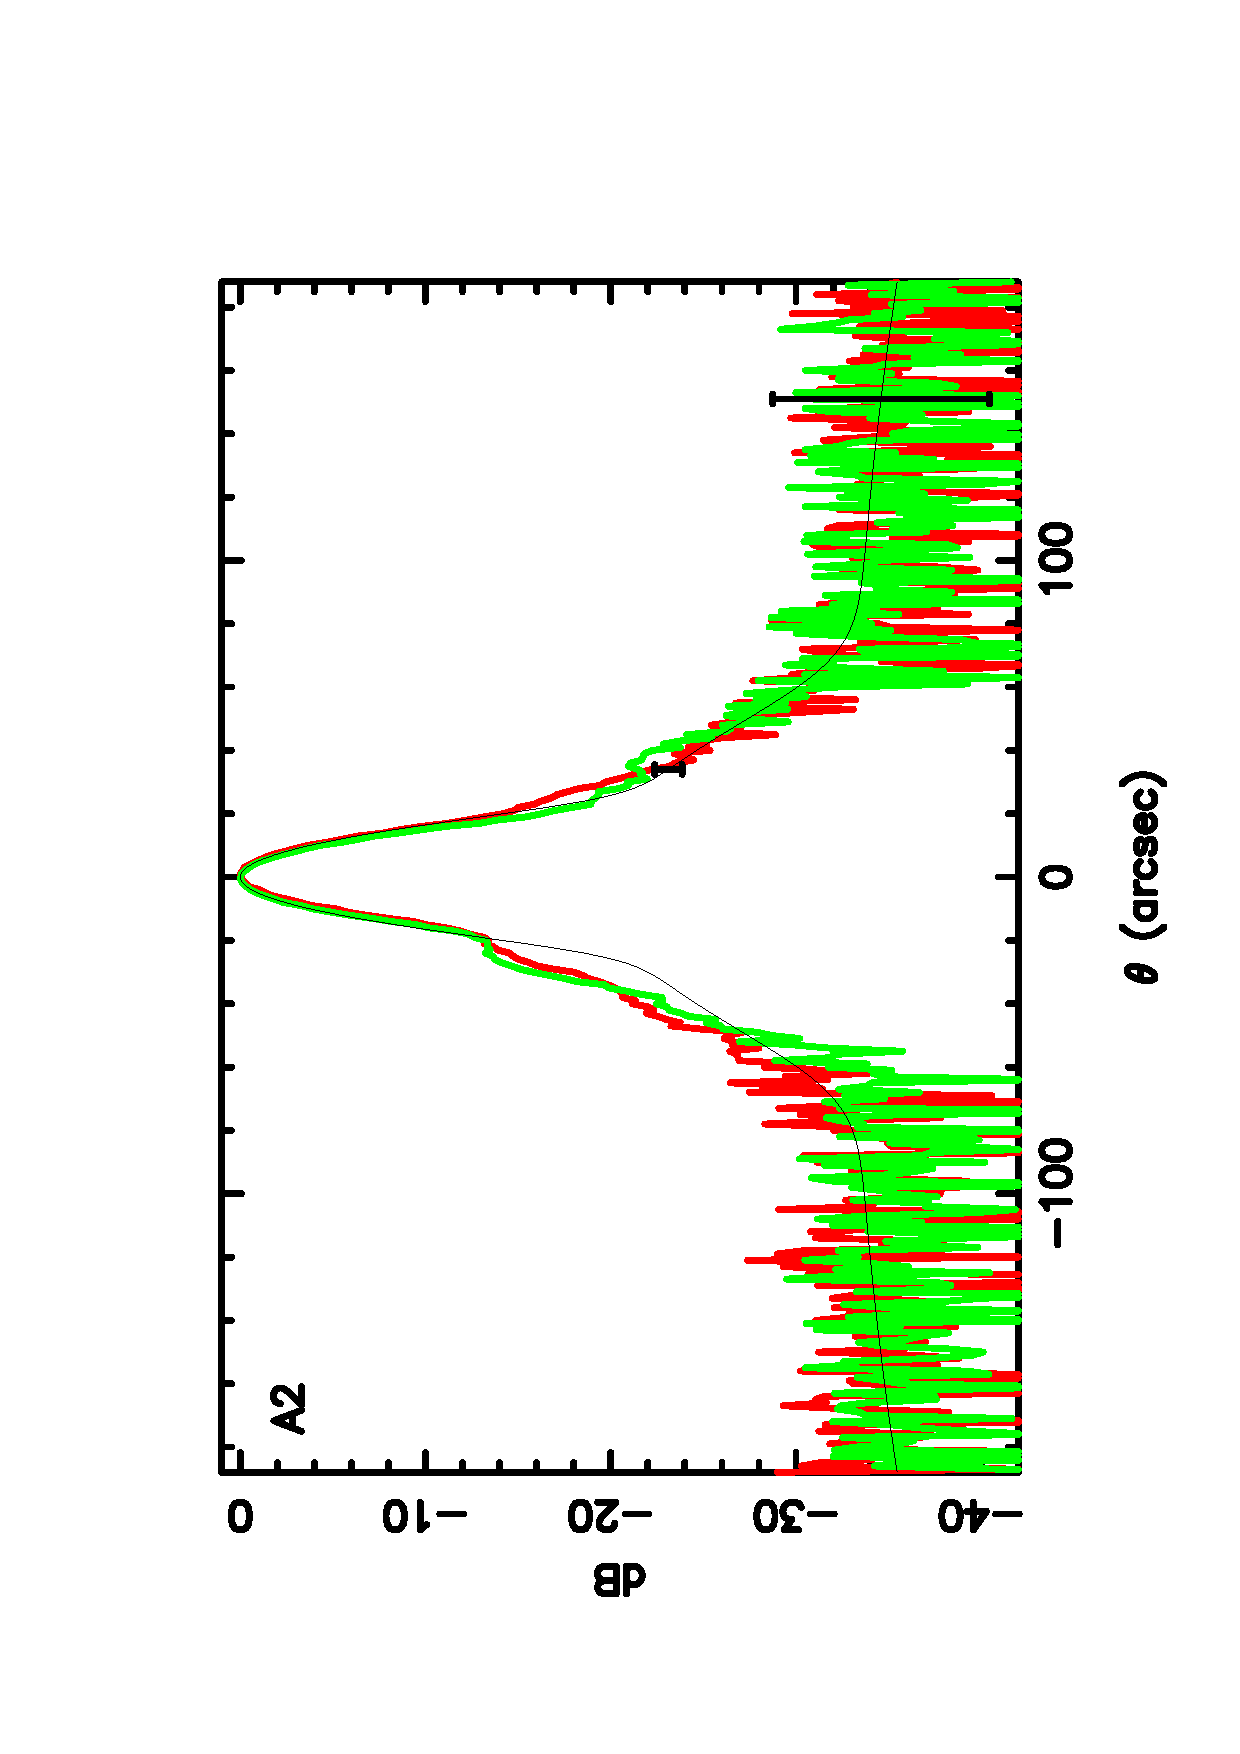
\includegraphics[clip, angle=-90, scale = 0.3]{Figures/Array_A2_dB.pdf}
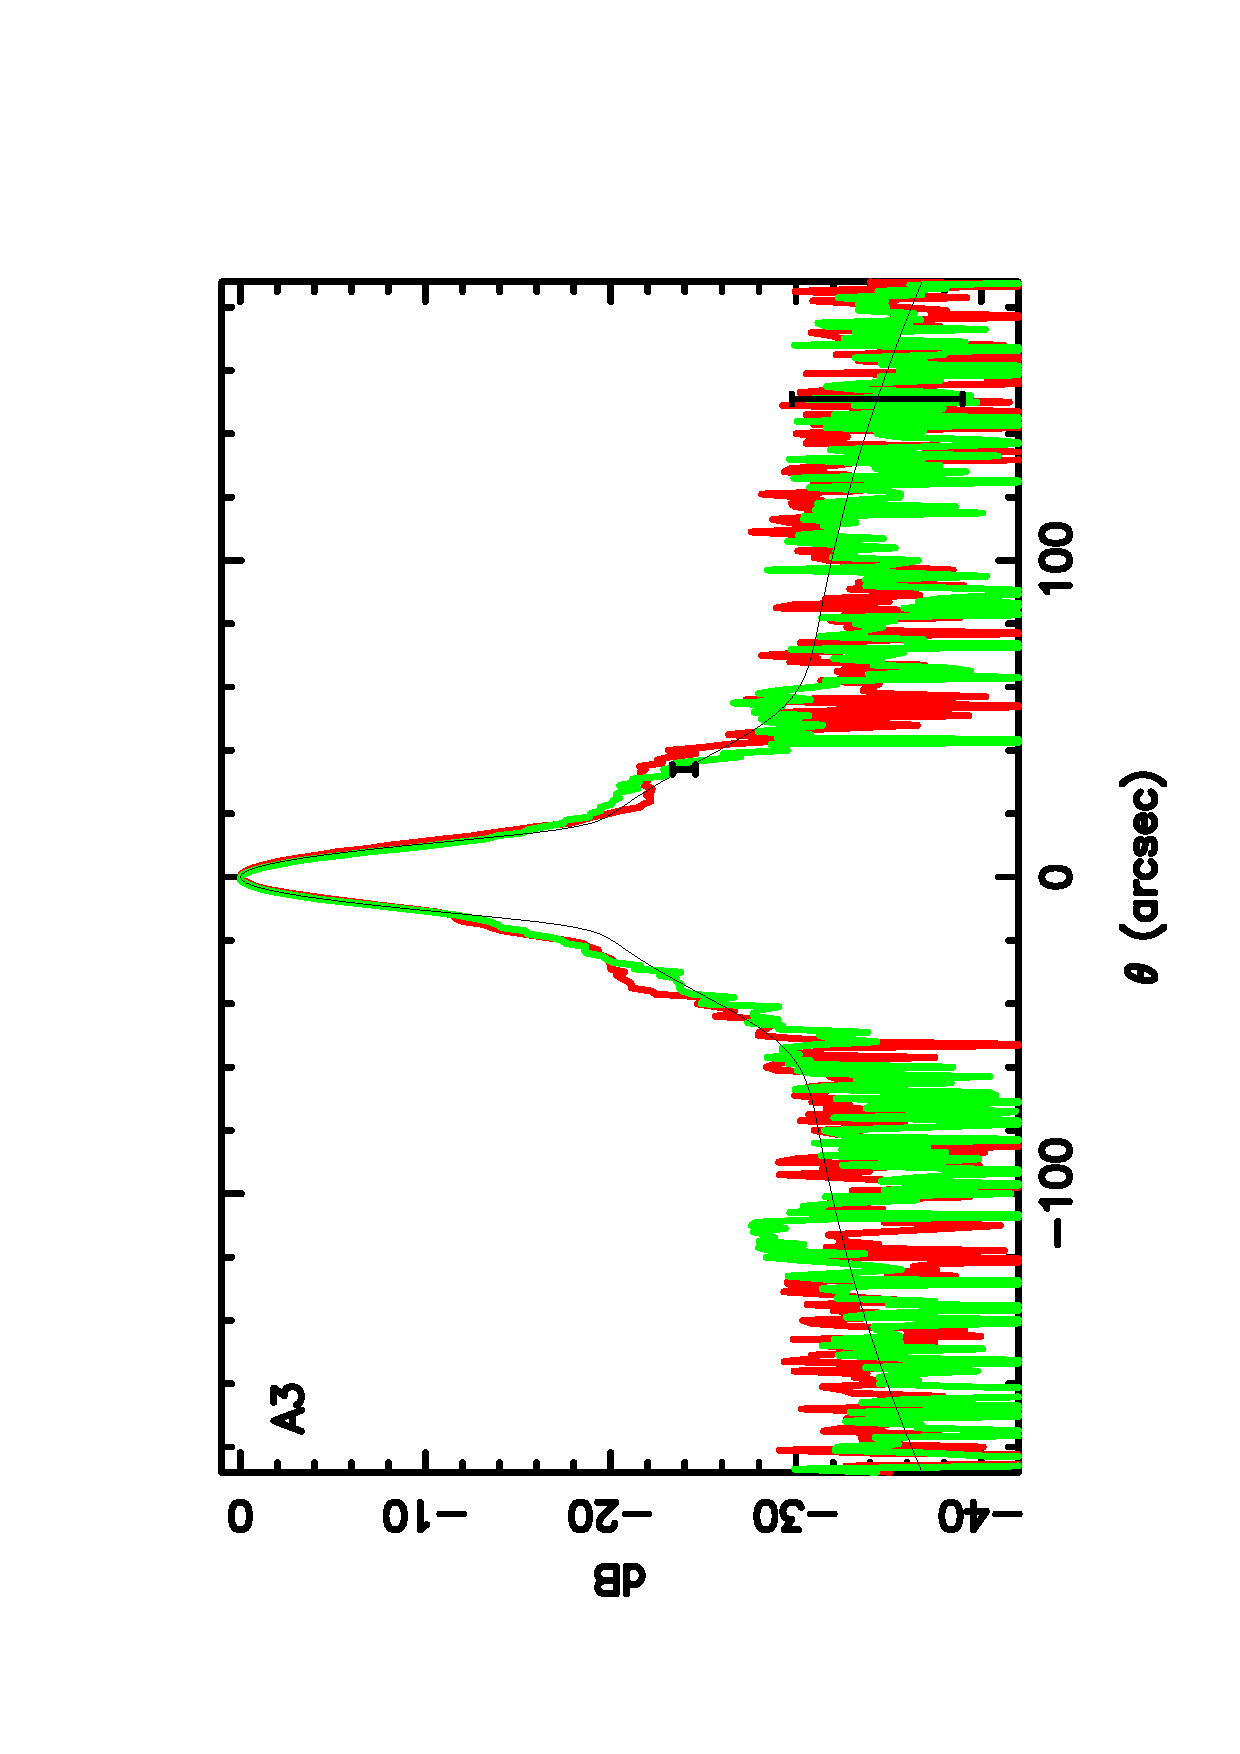
\includegraphics[clip, angle=-90, scale = 0.3]{Figures/Array_A3_dB.pdf}
\caption{Two orthogonal cuts through the beam are shown in red and green and a best fit model made
of three Gaussians is superimposed in black. These cuts were obtained from the high quality map of Uranus on 2017 January 25th.
The main beam starts to depart from the first Gaussian at -12dB. }
\label{fig:beam_dB3}
\end{center}
\end{figure}

The Iram 30-m beam as seen with NIKA2 is shown in
Fig. \ref{fig:beam_db} by means of two orthogonal cuts through Uranus
from a high quality map obtained on 2017 January 25th in excellent conditions
(low opacity $\tau_{225}=0.08$ and elevation $46^{\circ}$).
A model made of three Gaussians centered on the source peak was best
fit {\it by hand} to these cuts and the parameters are reported in
Table \ref{tab:3gauss} [PEUT-ETRE AVANTAGEUSEMENT REPLACED PAR VALEURS DE FLORIAN].
The main beam starts to depart from the first
Gaussian at the level of about -12dB for the three arrays.
We note that for the instrument EMIR on the radiotelescope,
this departure is about -20dB (Kramer, Penalver and Greve 2013).
From parameters in Table \ref{tab:3gauss}, one can estimate that
the source incident power is split about equally between the main beam
and the error beam at 1mm, and these fractions are 70\% and 30\% at 2mm, respectively.
This modelling uses the central
region   $180'' \times 180''$ in size with a uniform noise rms from
a larger area of 8' x 5' on the sky scanned with the arrays. It is expected
that the error beam extend beyond these limits.


\begin{table}
\centering 
\caption[]{Model parameters of the three Gaussian beam.}
\begin{tabular}{|l|l|l|l|l|l|l|}
\hline
               & \multicolumn{3}{c|}{A1 and A3} & \multicolumn{3}{c|}{A2}  \\
\hline
fwhm      & $11.25''$ & $45''$  & $250''$ & $17.75''$ & $56''$  & $420''$ \\
amplitude & 0.984     & 0.015   & 0.0005   &  0.9875   & 0.011   &  0.0005\\
\hline
\end{tabular}
\label{tab:3gauss}
\end{table}


\subsubsection{Beam profile}

\begin{figure*}[h!]
\centering
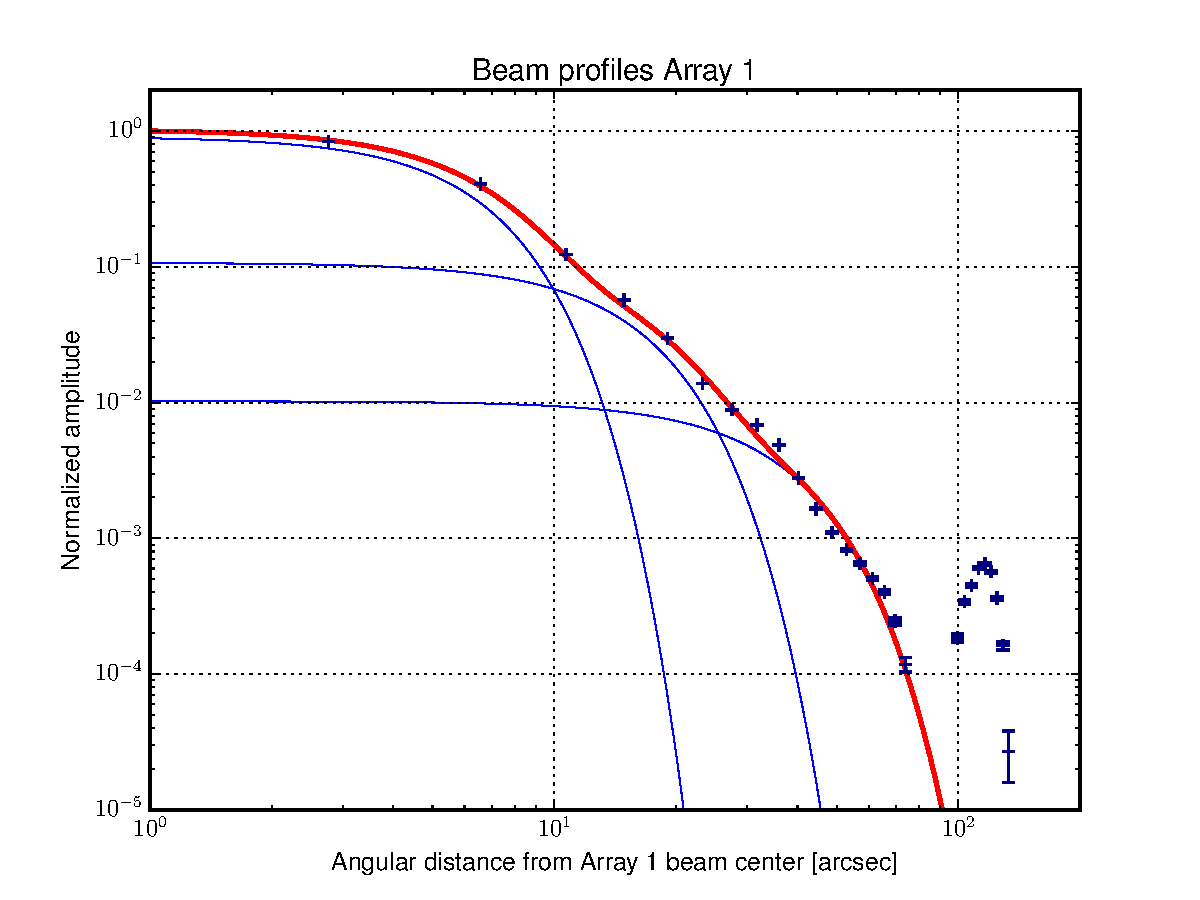
\includegraphics[height=6cm]{Figures/Beam_profiles_A1_FR.pdf}
\hspace{0.5cm}
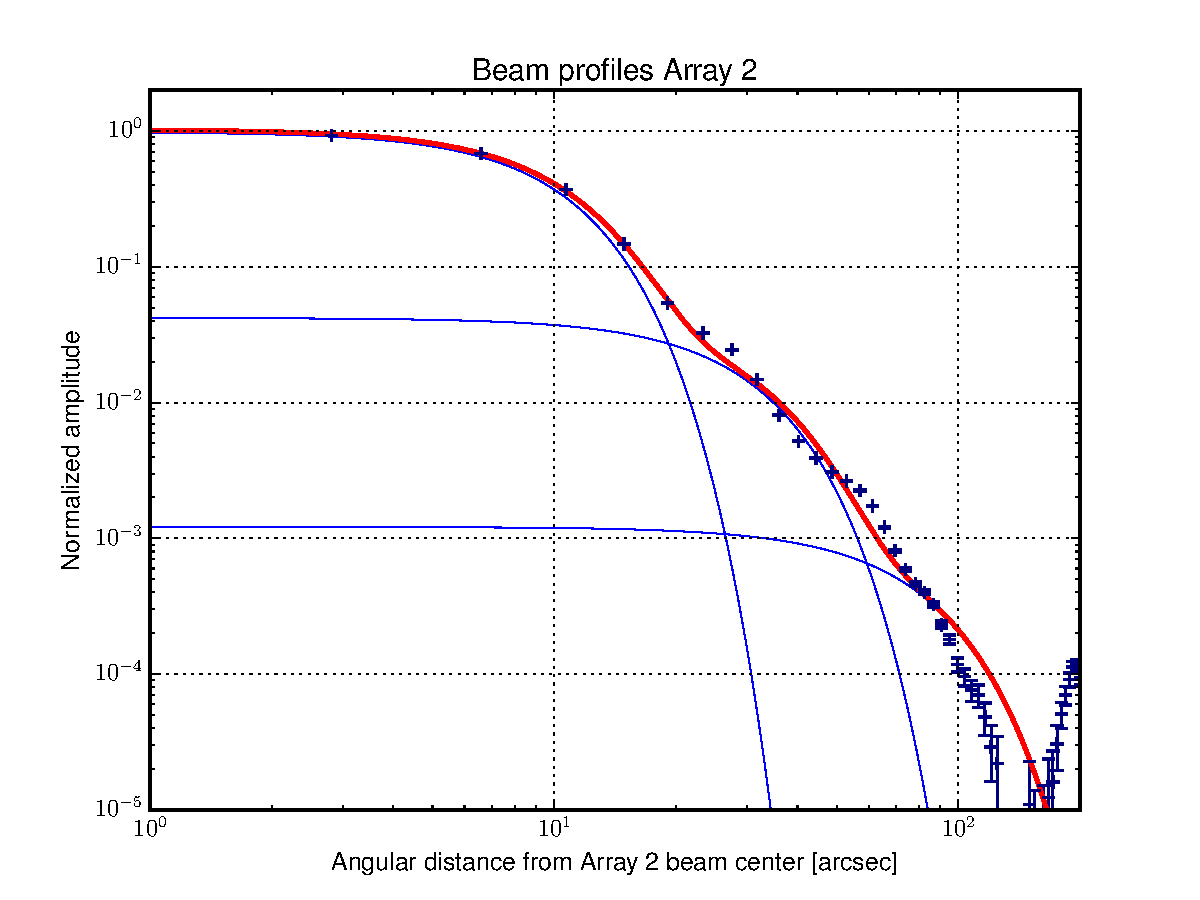
\includegraphics[height=6cm]{Figures/Beam_profiles_A2_FR.pdf}
\hspace{0.5cm}
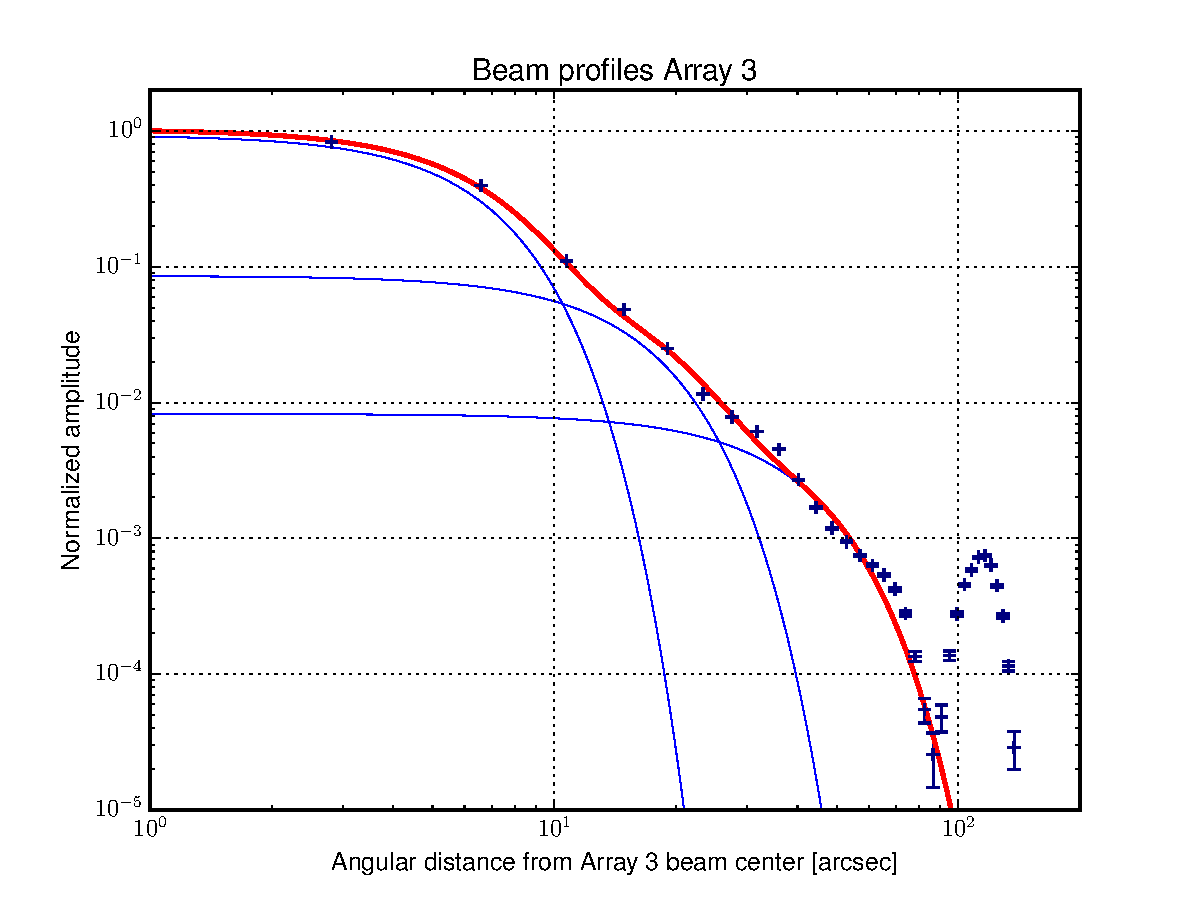
\includegraphics[height=6cm]{Figures/Beam_profiles_A3_FR.pdf}
\caption{{\footnotesize Beam profiles for array 1, 2, and 3.}}
\label{fig:beam_profiles_3G}
\end{figure*}


\subsubsection{Beam efficiency}


%% [STABILITY]
%%________________________________________________________
\subsection{Stability of the beam pattern}

[A FAIRE:

  AJOUTER LES PLOTS DE STABILITE EN FONCTION DE ELEVATION, TAU

]



